\chapter{Hauptteil}

\section{Architektur der Applikation}

\begin{figure}
	\centering
	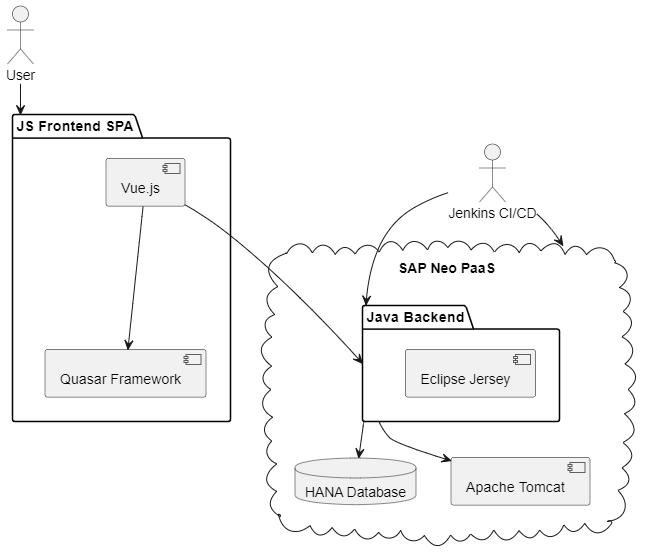
\includegraphics[width=.72\textwidth]{Bilder/architecture.png} 
	\caption{Die Abbildung zeigt die Architektur der Digital Heroes Lernplattform.}
	\label{fig:architecture}
\end{figure} 

Die Architektur der Web-App Digital Heroes mit den verschiedenen verwendeten Technologien
lässt sich in Frontend, Backend und DevOps unterteilen und 
ist in \autoref{fig:architecture} abgebildet. 
Es existieren zwei Instanzen der Architektur: ein Entwicklungs- und ein Produktivsystem. 

\subsubsection*{Frontend:}

Die Frontend-Anwendung der Digital Heroes Web-App ist als Single Page Application (SPA) konzipiert, 
die Vue.js und das Quasar Framework verwendet. 
Vue.js ist ein modernes JavaScript-Framework zum Erstellen von benutzerfreundlichen und reaktiven Webanwendungen.
Quasar ist ein weiteres Framework, das auf Vue.js aufbaut und zusätzliche Funktionen und Komponenten bereitstellt, 
um die Entwicklung von plattformübergreifenden Anwendungen zu erleichtern.
Vue.js nutzt die REST-API des Backends.

\subsubsection*{Backend:}

Das Backend der Web-App besteht aus einer Java-Anwendung, die Eclipse Jersey und Apache Tomcat verwendet. 
Eclipse Jersey ist eine Implementierung der JAX-RS-Spezifikation 
und ermöglicht die einfache Entwicklung von RESTful Web Services für Servlet Container. 
Apache Tomcat ist ein Servlet-Container, der als Webserver zum Bereitstellen von Java-Anwendungen dient
und das Java-Backend hostet.
Als Datenbank kommt die HANA-Datenbank zum Einsatz, die eine high-performance, in-memory relationale Datenbank ist 
und von SAP entwickelt wird. 
Das Java-Backend nutzt das Eclipse-Framework und die HANA-Datenbank um eine REST-API für das 
Vue.js-Frontend bereitzustellen. 

\subsubsection*{DevOps:}

Im Bereich der DevOps-Infrastruktur kommt Jenkins zum Einsatz, 
eine Open-Source-Automatisierungssoftware, 
die zur Implementierung von Continuous Integration und Continuous Deployment (CI/CD) verwendet wird. 
Jenkins ermöglicht die Automatisierung von Build- und Testprozessen sowie die Bereitstellung 
der Anwendung in einer kontrollierten und konsistenten Weise. 
Die Web-App wird auf der SAP Neo Platform-as-a-Service (PaaS) Cloud-Plattform gehostet, 
die eine skalierbare und einfach zu verwaltende Umgebung für die Bereitstellung 
und den Betrieb der Anwendung bietet.
Wird auf den Main-Branch des verwendeten Github-Respositories gepusht, bzw. eine Pull-Request gemerged,
startet Jenkins den CI/CD-Prozess und testet und deployed das neue Backend/Frontend auf der Entwicklungsinstanz. 
Änderungen im Frontend werden zudem direkt auf dem Produktivsystem deployed. 
Für Änderungen des Backends im Produktivsystem kann in SAP Neo ein neuer Release erzeugt werden, 
bei dem das Java-Backend der Entwicklungsinstanz auf das Produktivsystem kopiert wird. 


\section{Ist-Situation und warum die problematisch ist}

Das Entwickler-Team ist auf Deutschland und Australien aufgeteilt, 
was zu Kommunikationsschwierigkeiten und unterschiedlichen Arbeitszeiten führt. 
Dies erschwert die Zusammenarbeit und kann die Qualität der Software und die Effizienz 
der Entwicklungsprozesse beeinträchtigen.

Es gibt keine fest vorgegebenen Release-Zyklen; Releases finden nur statt, 
wenn ein neues Feature fertig ist. Dies kann zu unvorhersehbaren und unregelmäßigen Updates führen,
wodurch die Planung und das Management des Projekts schwieriger werden.
Außerdem werden Features möglicherweise nicht ausreichend vor einem Release getestet.

Releases werden oft freitags durch das australische Team durchgeführt. 
Dies ist problematisch, weil das Team in Australien möglicherweise nicht verfügbar ist, 
um eventuell auftretende Probleme sofort zu beheben, was zu längeren Ausfallzeiten führt. 
Das deutsche Team muss dann freitags die Probleme beheben oder einen Roll-Back veranlassen, 
wenn die Probleme zu groß sind. Insbesondere muss sich das deutsche Team aber erst 
in den Code des australischen Teams einlesen, was das Beheben der Fehler viel ineffizienter 
gestaltet, als wie wenn das australische Team diese Fehler beheben würde.

Es gibt keinerlei automatisierte Tests. Das bedeutet, 
dass die Qualität der Software nicht kontinuierlich überprüft wird, 
wodurch Fehler erst spät oder gar nicht entdeckt werden. Dies erhöht das Risiko drastisch, 
dass Fehler in die Produktion gelangen, was zu einer schlechteren Benutzererfahrung führt.

Viele Bugs gelangen in die Produktionsumgebung, 
was häufig auf die fehlenden Tests zurückzuführen ist, 
wodurch oft Hot-Fixes notwendig sind. Dies zeigt, 
dass der Entwicklungsprozess und die Qualitätssicherung unzureichend sind 
und die Softwarequalität leidet. Außerdem sind die Hot-Fixes selbst ungetestet 
und sehr überhastet erstellt worden, was wiederum zu mehr Bugs führen kann. 
Auch betreffen diese Bugs gelegentlich völlig andere Teile des Systems und fallen nicht sofort auf.
Zu allem Überfluss werden diese Hot-Fixes mit diesen gefährlichen Bugs direkt auf das Produktiv-System 
deployed. 

Der CI/CD-Prozess für das Deployment auf der Entwicklungsinstanz dauert 15 Minuten. 
Das ist eine lange Wartezeit, die den Entwicklungsprozess verlangsamt und zu einer geringeren Produktivität führt.
Zur Verschlimmerung der Lage kann das Backend nicht auf dem lokalen Rechner gestartet werden, 
da die HANA-Datenbank nicht lokal gehostet werden kann und kein Mock existiert. 
Dies erschwert die lokale Entwicklung und das Testen, 
was die Effizienz der Entwickler stark beeinträchtigt und die Qualität der Software gefährdet, 
da Neuerungen weniger getesetet werden, weil der Testprozess so frustrierend für die Entwickler ist.

Die Codequalität ist in einem schrecklichen Zustand: Viele duplikative Code-Stücke, 
wenig Struktur und keine Aufteilung der Architektur in Schichten. 
Es wird immer gegen Implementierungen programmiert, anstatt gegen Abstraktionen. 
Dies führt zu einer schlechteren Wartbarkeit, schlechterer Lesbarkeit, 
erschwert das Testen, da Mocks und Fakes nicht möglich sind,  
erhöht die Fehleranfälligkeit und erschwert die Einarbeitung neuer Teammitglieder, 
was insbesondere in dem Projekt ein Problem ist, da oft Studenten hier arbeiten, 
die nicht für lange Zeit eingebunden sind und dadurch hohe Fluktation besteht. \\
Desweiteren ist der Code ist oft fehleranfällig und unleserlich, 
zum Beispiel durch 40-50 Zeilen lange, 
verschachtelte SQL-Statements, die viel Code-Duplikate enthalten. 
Dies führt zu einer schlechteren Wartbarkeit und macht es schwieriger, 
Fehler zu erkennen und zu beheben, da oft nicht alle Duplikate angepasst werden.

Es gibt keine Code-Reviews, was bedeutet, dass keine systematische Überprüfung der Codequalität 
stattfindet. Dies erhöht die Wahrscheinlichkeit von Fehlern und mindert damit die Qualität der Software.

Obwohl ein Kanban-Board mit Tasks und Prioritäten verwendet wird, 
gibt es kein Sprint-Planning und kein Sprint-Review. 
Dies führt zu einer schlechteren Planung und Kontrolle der Arbeit 
und beeinträchtigt die Effizienz des Entwicklungsprozesses, weil keine klarere Absteckung der 
Aufgaben stattfindet und nicht bewertet wird, wie der vorangegangene Sprint lief.

Die Scrum-Meetings finden zweimal pro Woche statt, 
aber mit der ganzen Abteilung (nicht nur Entwickler, sondern auch Designer, Manager, Content-Moderatoren usw.). 
Dadurch werden diese Meetings sehr ineffizient, 
da nicht alle Teilnehmer direkt am Entwicklungsprozess beteiligt sind. 
Dies führt zu einer schlechteren Kommunikation und Koordination innerhalb des Entwicklerteams 
und verlangsamt den Entwicklungsprozess enorm, da die Mitglieder in dem Meeting gebunden sind, 
obwohl ein Großteil der Inhalte nicht relevant für das jeweilige Mitglied sind. 
Dadurch wird viel Zeit verschwendet.

Insgesamt sind die identifizierten Probleme im Bereich des Software-Qualitäts-Managements
und Entwicklungsprozesse ein erhebliches Hindernis für die Erreichung einer 
hohen Softwarequalität und einer effizienten Arbeitsweise. Um die Situation zu verbessern, 
müssen die genannten Probleme adressiert und Lösungen gefunden werden, 
die zu einer besseren Organisation, Kommunikation und Qualitätssicherung führen.

\section{Mögliche Ursachen für die identifizierten Probleme}

Die geschilderten Probleme in Bezug auf das Software-Qualitäts-Management 
und den Entwicklungsprozess sind vielfältig und komplex. Es gibt mehrere mögliche Gründe, 
die zu diesen Schwierigkeiten geführt haben. Um diese Probleme nachhaltig zu lösen, 
müssen die Gründe verstanden werden, die dazu geführt haben, ansonsten werden nur 
Symptome behandelt und die Probleme nicht an der Wurzel angegangen. 
Eine kritische Untersuchung der Situation zeigt folgende mögliche Ursachen:

Unerfahrene Projektleitung: Eine der Hauptursachen für die identifizierten Probleme 
ist eine unerfahrene oder teilweise auch überforderte Projektleitung. 
Da die festangestellte Projektleitung wenig Erfahrung im Bereich Softwareentwicklung 
und Projektmanagement hat, führt dies dazu, dass sie die bestehenden Probleme nicht versteht 
oder realisiert. Dies führt zu einer unzureichenden Organisation, 
fehlender Prozesskontrolle und wenig Vertsändnis für Ressourcenaufwand, welcher für Qualitätssicherung 
eingesetzt wird.

Hoher Anteil unerfahrener Studenten: Die schlechte Qualität der Software 
und der Entwicklungsprozesse könnte auch auf den hohen Anteil unerfahrener Studenten zurückzuführen sein, 
die in der Abteilung arbeiten. Da diese Studenten nur für eine begrenzte Zeit
im Projekt tätig sind und nicht die erforderliche Erfahrung haben, 
kann dies zu einer hohen Mitarbeiterfluktuation und einer unzureichenden Kontinuität in der Entwicklung führen. 
Dies wirkt sich negativ auf die Qualität der Software und die Effizienz der Entwicklungsprozesse aus.

Fehlende Verantwortung und Initiative: Ein weiterer Grund für die identifizierten Probleme könnte sein, 
dass sich keines der Teammitglieder verantwortlich fühlt, die Probleme zu adressieren und zu verbessern. 
Dies kann auf mangelnde Kommunikation (insbesondere zwischen deutschem und australischem Team), 
fehlende Anreize oder eine unklare Rollenverteilung 
innerhalb des Teams zurückzuführen sein. Wenn niemand das Gefühl hat, 
für die Qualität der Software und die Effizienz der Entwicklungsprozesse verantwortlich zu sein, 
wird es schwierig sein, die Situation nachhaltig zu verbessern.

Kommunikationsschwierigkeiten: Die Aufteilung des Entwicklerteams auf verschiedene Standorte, 
wie Deutschland und Australien, kann zu Kommunikationsschwierigkeiten führen. 
Zeitverschiebung, kulturelle Unterschiede und eine eingeschränkte Möglichkeit 
für persönliche Treffen führen dazu, dass Missverständnisse entstehen und Entscheidungen 
nicht effektiv getroffen werden.

Hoher Druck durch Nutzeranforderungen: Die Nutzer fordern häufig schnell neue Features, 
was den Druck auf die Studenten erhöht, diese Anforderungen umzusetzen. 
Da die Studenten möglicherweise nicht in der Lage sind, 
"nein" zu sagen oder Prioritäten angemessen zu setzen, 
kann dies zu einer Vernachlässigung von wichtigen Aspekten wie Qualitätssicherung, 
Testentwicklung und Code-Reviews führen. 

Fokus auf Feature-Entwicklung statt Testentwicklung: Die studentischen Entwickler legen den Fokus eher auf 
die Implementierung neuer Features, anstatt auf das Schreiben von Tests, 
da das Erstellen neuer Funktionen als "spannender" oder "produktiver" wahrgenommen wird. 
Außerdem wird durch die fehlende Erfahrung das Schreiben von Tests und anderen 
Qualitätssicherungsmaßnahmen als eher unwichtig eingeschätzt. 

Mangel an Vollzeitentwicklern: Da es keine Vollzeitentwickler oder Senior Development-Experten gibt,
wird die Entwicklungsleitung nicht durch einen erfahrenen Entwickler übernommen, 
der die nötige Führung für die jungen studentischen Junior Entwickler bieten könnte.

\section{Grundlagentheorie für Optimierung der Ist-Situation und identifizierten Probleme}

In diesem Abschnitt wird die Theorie aus der Softwarequalitäts-Vorlesung 
dargelegt und erklärt, die für die Optimierungen des gegebenen 
Fallbeispiels der Digital-Heroes-Plattform notwendig ist. 
Zudem wird kurz erwähnt, wofür jeder Theoriepunkt später verwendet wird, 
um den Überblick zu verbessern. 

\subsection*{Das magische Dreieck}

Zunächst soll das magische Dreieck des Projektmanagements erklärt werden, 
da es später genutzt wird, um die Priorisierung besser zu bestimmen. Es ist ein grundlegendes Konzept, 
das die drei wichtigsten Faktoren eines Projekts darstellt: Zeit, Kosten und Umfang. 
Das magische Dreieck zeigt die Beziehung zwischen diesen Faktoren und wie sie sich gegenseitig beeinflussen.

\textbf{Zeit:} Zeit bezieht sich auf den Zeitrahmen, innerhalb dessen das Projekt abgeschlossen werden muss. 
Bei Digital Heroes sind das bspw. bis wann neue Features erstellt sein sollen. \\
\textbf{Kosten:} Kosten beziehen sich auf das Budget und die Ressourcen, die für das Projekt zur Verfügung stehen. 
Im Anwendungsbeispiel sind das neben dem Budget auch die Entwickler, da für einige der Studenten, wie z.B. 
mich als dualer Student, die Abteilung nicht bezahlen muss. \\
\textbf{Umfang/Scope:} Der Umfang oder auch Scope bezieht sich auf die Gesamtheit der Arbeit, 
die innerhalb des Projekts geleistet werden muss.
Bei Digital Heroes wäre das also z.B. die Anzahl und Größe der neuen Features, die gefordert wird. 
Im Umfang sind aber auch Maßnahmen zur Qualitätssicherung enthalten.  

Das magische Dreieck zeigt, dass Änderungen an einem Faktor das gesamte Projekt beeinflussen können. 
Zum Beispiel kann eine Verzögerung im Zeitplan, z.B. durch Krankheit eines Entwicklers, zu erhöhten Kosten führen, 
da zusätzliche Arbeitsstunden für die restlichen Entwickler erforderlich sein können. 
Oder eine Erweiterung des Projektumfangs, z.B. aufwendigere oder mehr Features, kann dazu führen, 
dass mehr Budget und Ressourcen benötigt werden, 
um das Projekt innerhalb des Zeitrahmens abzuschließen.
Um die Qualität des Projektes sicherzustellen, sollte auf ein ausgeglichenes Verhältnis der drei Faktoren 
geachtet werden, sodass man sich in der 'Mitte' des magischen Dreiecks bewegt. 


\subsection*{SCRUM}




zuerst magisches dreieck und soll helfen gegen priorisierung von aufgaben und kosten usw
für weniger stress bei studenten. Studenten sind schon günstig. erklärung auf beispiel beziehen.